\documentclass[a4paper,10pt]{article}
\usepackage{My_math_package}



\title{MATH868C - Several Complex Variables}
\author{Haoran Li}
\date{2020 Fall}

\makeindex[columns=2, title=Index, intoc] % Create the index

\begin{document}\sloppy % reduce overlong words

% Maketitle
\begin{titlepage}
\begin{center}
\vspace*{1cm}
\LARGE
\textbf{MATH868C - Several Complex Variables} \\
\vspace{2cm}
\begin{center}
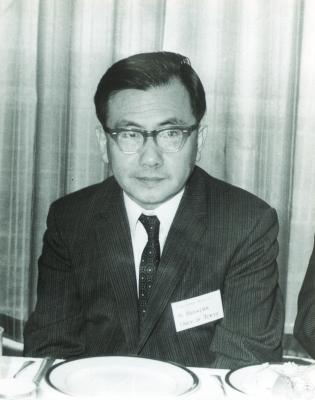
\includegraphics[width=0.5\textwidth]{Pictures/Kodaira_Kunihiko.jpg}
\end{center}
\vspace{2cm}
\normalsize
Taught by \texttt{Richard A. Wentworth} \\
Notes taken by \texttt{Haoran Li} \\
2020 Fall \\
\vspace{2cm}
Department of Mathematics\\
University of Maryland\\
\end{center}
\end{titlepage}

\tableofcontents
\newpage

\section{Review}
\subfile{Review.tex}
\newpage

\section{Runge's theorem}
\subfile{Runge's_theorem.tex}
\newpage

\section{Subharmonic functions}
\subfile{Subharmonic_functions.tex}
\newpage

\section{Almost complex structure}
\subfile{Almost_complex_structure.tex}
\newpage

\section{Hartogs theorem}
\subfile{Hartogs_theorem.tex}
\newpage

\section{Pseudoconvexity}
\subfile{Pseudoconvexity.tex}
\newpage

\section{H\"ormander's $L^2$ estimate}
\subfile{Hormander's_L2_estimate.tex}
\newpage

\section{Kahler metrics}
\subfile{Kahler_metrics.tex}
\newpage

\section{Solving $\bar\partial$ equation}
\subfile{Solving_dbar.tex}
\newpage

\section{Proper mapping theroems}
\subfile{Proper_mapping_theroems.tex}
\newpage

\begin{thebibliography}{}

\bibitem{An Introduction to Complex Analysis in Several Variables - Hormander} 
\textit{An Introduction to Complex Analysis in Several Variables} - Lars H\"ormander



\end{thebibliography}

\printindex
\newpage

\end{document}